
In the previous sections, we predict reactions to a turn based on the topics present in the turn. We find that we can do this reasonably well for some types of prediction, and also learn what topics contribute most to certain reactions.

We can also ask what topics cause an individual user to react, rather than users in general. The label for prediction then becomes that user's reaction, and the features become the topics present in the discussion at the time of the reaction.

However, since we are now working at the individual level, we can also use features based on a user's responses to the ReactLabs survey questions, which we will call "user features." These include questions such as gender and political party, and also questions that ask the user to indicate agreement with one party or another on specific issues with a value between 0 and 100.

We are primarily interested in 1.) how well we can predict user reactions given user features and topic features, and 2.) how much topic features contribute to classification accuracy. Topic features are determined based on the turn in which the reaction occurs. We use features derived from both LDA topics and the Boydstun labeled topics. Labels are the 12 possible user reactions ("$Obama|Romney|Moderator : Agree|Disagree|Spin|Dodge$"). We use 10,000 reactions for 10-fold cross-validation.

\begin{table*}[H]
\begin{centering}
\begin{tabular}{ l | l | l | l }
Classifier & User features only & User + LDA & User + Boydstun \\
\hline
Decision Tree & \textbf{0.389} (.018) & \textbf{0.397} (.016) &  \textbf{.388} (.014) \\
Maximum Entropy & \textbf{.452} (.019) & \textbf{0.517} (.012) &  \textbf{.508} (.022) \\
Naive Bayes & \textbf{.443} (.020) & \textbf{0.481} (.012) &  \textbf{.460} (.013) \\
\end{tabular}
\caption{User reaction classification: accuracy and standard deviation}
\end{centering}
\end{table*}

We also plot confusion matrices using the best-performing classifier for both user features alone and user features combined with topic features.

\begin{figure}[H]
	\centering
	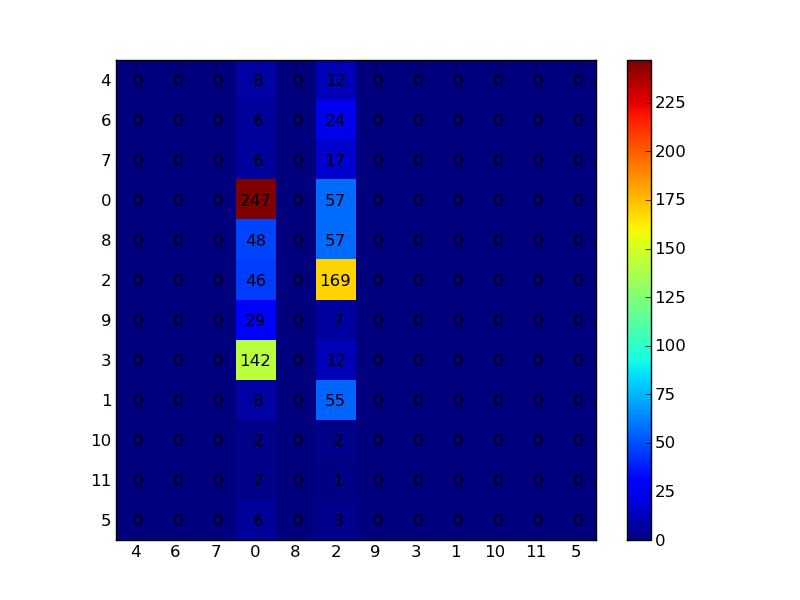
\includegraphics[scale=0.35]{Figures/no_topic_features_confusion.png}
	\caption{Confusion Matrix: Classification with user features only}
	\label{fig:useronlyconfusion}
\end{figure}

\begin{figure}[H]
	\centering
	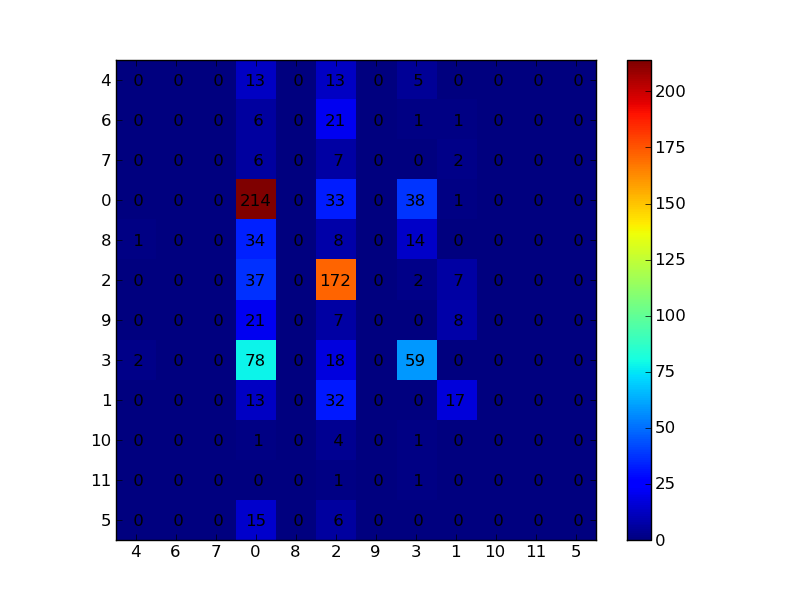
\includegraphics[scale=0.35]{Figures/boydstun_confusion.png}
	\caption{Confusion Matrix: Classification with user and topic features}
	\label{fig:boydstunconfusion}
\end{figure}


\begin{table}[H]
\begin{centering}
\begin{tabular}{ l | l | l | l }
 Code & Topic & Code & Topic \\
\hline
4 & Moderator:Agree & 9 & Romney:Dodge \\
6 & Obama:Spin & 3 & Romney:Disagree \\
7 & Obama:Dodge & 1 & Obama:Disagree \\
0 & Obama:Agree & 10 & Moderator:Spin \\
8 & Romney:Spin & 11 & Moderator:Dodge \\
2 & Romney:Agree & 5 & Moderator:Disagree \\
\end{tabular}
\caption{Topic code key}
\end{centering}
\end{table}

As expected, using topic-based features in addition to user features improves classification accuracy. The maximum entropy classifier shows the greatest improvement, increasing from $45.2\%$ accuracy to $51.7\%$ accuracy.

This is an interesting result, since the maximum entropy classifier is the one classifier that makes no independence assumptions between the features. The increase in accuracy suggests that it does a better job of integrating the user features with the topic features. For instance, the maximum entropy classifier might be more capable of classifying the reaction of a user who indicates a certain topic is more important to him during a turn in which that topic is present.

From the confusion matrices, one can see that the majority of predictions fall into labels 0 and 2, corresponding to "Obama:Agree" and "Romney:Agree." In Figure \ref{fig:useronlyconfusion}, labels for "Romney:Disagree" are often confused with labels for "Obama:Agree." This makes sense, since a user who disagrees with Romney most likely agrees with Obama. Including topic features results in more predictions of labels 3 and 1, "Obama:Disagree" and "Romney:Disagree" (Figure \ref{fig:boydstunconfusion}).